\begin{figure}
  \centering
  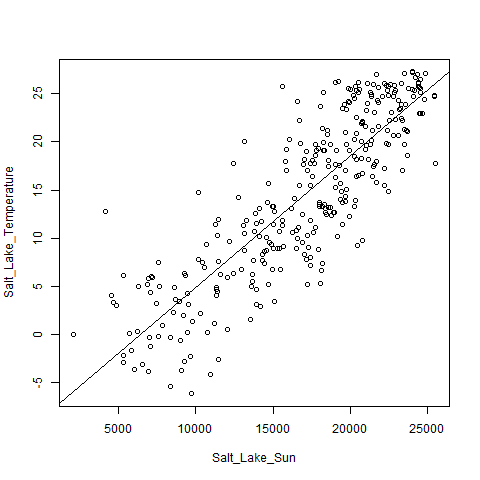
\includegraphics[width=7cm]{../data/img/Temp_vs_sun.PNG}
  \caption{Salt Lake City Temperature versus Sun}
  \label{fig:temp_vs_sun}
\end{figure}

\begin{figure}
  \centering
  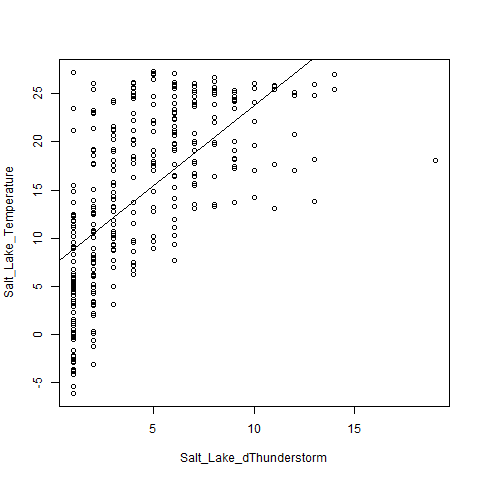
\includegraphics[width=7cm]{../data/img/Temp_vs_dThunderstorm.PNG}
  \caption{Salt Lake City Temperature versus Days with Thunderstorms}
  \label{fig:temp_vs_dthunderstorms}
\end{figure}

\begin{figure}
  \centering
  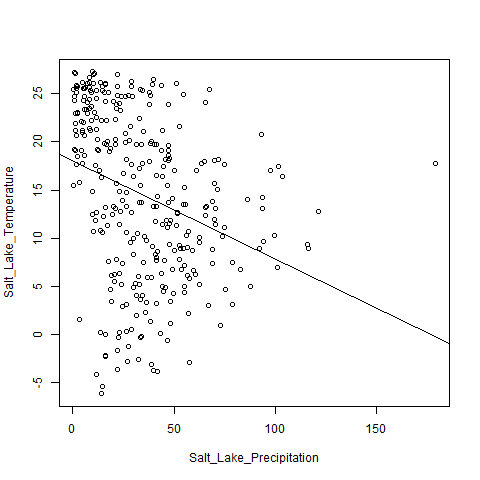
\includegraphics[width=7cm]{../data/img/Temp_vs_Precipitation.PNG}
  \caption{Salt Lake City Temperature versus Precipitation}
  \label{fig:temp_vs_precipitation}
\end{figure}

\begin{figure}
  \centering
  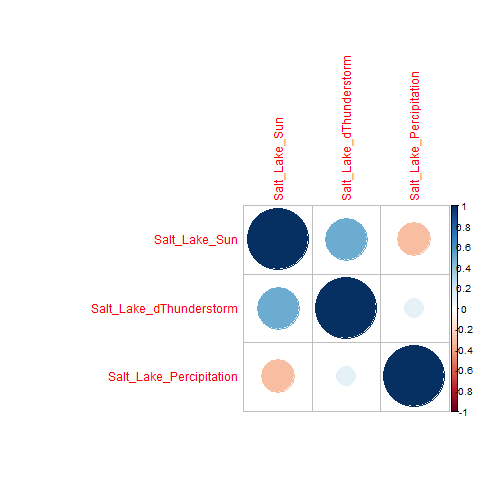
\includegraphics[width=7cm]{../data/img/correlation_plot.PNG}
  \caption{Correlation plot of chosen dependent variables}
  \label{fig:correlation_plot}
\end{figure}

\begin{table}[ht]
 \begin{centering}
 \begin{tabular}{|c|c c c c c|} 
 \hline
 $$ & & & & Days with & \\ [0.5ex] 
 & Temperature & Intercept & Minutes of Sun & Thunderstorms & Precipitation \\
 \hline\hline
 $P_{Shapiro}$ & $2.662\times 10^{-8}$ & -- & $6.845\times 10^{-9}$ & $9.438\times 10^{-15}$ & $2.817\times 10^{-12}$ \\ 
 \hline
 $\beta$ & -- & -5.261 & $1.041\times 10^{-3}$ & 0.8471 & $-4.800\times 10^{-2}$ \\ 
 \hline
 $P(>|t|)$ & -- & $2.30\times 10^{-8}$ & $< 2.00\times 10^{-16}$ & $< 2.00\times 10^{-16}$ & $< 2.91\times 10^{-7}$ \\ 
 \hline
 \end{tabular}
 \caption{Multiple Linear Regression for Predicting Temperature (Adjusted $R^{2} = 0.7969$, $n = 321$)}
 \label{tab:lin_regression}
 \end{centering}
\end{table}

\begin{table}[ht]
 \begin{centering}
 \begin{tabular}{|c|c c c|} 
 \hline
  \# Variables & Minutes of Sun & Days with Thunderstorms & Precipitation \\
 \hline
 1 & * & & \\
  \hline
 2 & * & * & \\ 
  \hline
 3 & * & * & *\\ 
 \hline
 \end{tabular}
 \caption{Optimal Subset selection for Multiple Linear Regression}
 \label{tab:optimal_selection}
 \end{centering}
\end{table}

\begin{table}[ht]
 \begin{centering}
 \begin{tabular}{|c|c c c|} 
 \hline
   & Model 1 & Model 2 & Model 3 \\
 \hline
 AIC & 1875.498 & 1805.823 & 1781.139 \\
  \hline
 BIC & 1886.812 & 1820.909 & 1799.996 \\ 
  \hline
 Adjusted $R^{2}$ & 0.7258 & 0.78 & 0.7969\\ 
 \hline
 \end{tabular}
 \caption{Model Comparisons for Multiple Linear Regression}
 \label{tab:model_info}
 \end{centering}
\end{table}

\begin{table}[ht]
 \begin{centering}
 \begin{tabular}{|c|c c c c c|} 
 \hline
 $$ & & & & Days with & \\ [0.5ex] 
 & Temperature & Intercept & Minutes of Sun & Thunderstorms & Precipitation \\
 \hline\hline
 $P_{Shapiro}$ & $3.259\times 10^{-7}$ & -- & $2.592\times 10^{-7}$ & $2.011\times 10^{-13}$ & $1.88\times 10^{-8}$ \\ 
 \hline
 $\beta$ & -- & -4.795 & $1.037\times 10^{-3}$ & 0.8541 & $-6.308\times 10^{-2}$ \\ 
 \hline
 $P(>|t|)$ & -- & $4.85\times 10^{-6}$ & $< 2.00\times 10^{-16}$ & $< 2.00\times 10^{-16}$ & $< 1.94\times 10^{-8}$ \\ 
 \hline
 \end{tabular}
 \caption{Multiple Linear Regression for Predicting Temperature with Missing Data (Adjusted $R^{2} = 0.797$, $n = 260$)}
 \label{tab:lin_regression_missing_data}
 \end{centering}
\end{table}

\begin{table}[ht]
 \begin{centering}
 \begin{tabular}{|c|c c c|} 
 \hline
   & Model 1 & Model 2 & Model 3 \\
 \hline
 AIC & 1530.985 & 1481.879 & 1451.769 \\
  \hline
 BIC & 1541.667 & 1496.121 & 1469.572 \\ 
  \hline
 Adjusted $R^{2}$ & 0.7226 & 0.7713 & 0.797\\ 
 \hline
 \end{tabular}
 \caption{Model Comparisons for Multiple Linear Regression with Missing Data}
 \label{tab:model_info_missing_data}
 \end{centering}
\end{table}